\section{Introduction}

\subsection{Motivation}

Almost 70 years after MADALINE \cite{adaline}, the first successful application of an artificial neural network that predicted and corrected bit streams traversing a phone line, the interest in artificial neural networks and Artificial Intelligence (AI) in general has grown exponentially. Parallel to the ever-improving research, industry applications of neural networks have been numerous, ranging from stock market predictions \cite{smp} to self-driving cars as early as 1989 \cite{alvinn}. These applications continue to create new business opportunities and thus investments have been flowing into AI over the past years at unprecedented levels. Moreover, this trend is predicted to continue with enterprise market revenue expected to be multiplied by 20 by 2025; see Fig.~\ref{fig:ai-proj}. As a direct consequence, research is prolific as observed in Fig.~\ref{fig:ai-papers} and funding has grown significantly. Indeed, The European Union (EU) is even encouraging these investments and is aiming to reach 20 billion euros worth of both public and private investments in AI in 2020. \cite{ai-invest}.

\begin{figure}[!ht]
   \centering
   \begin{subfigure}[b]{0.5\textwidth}
       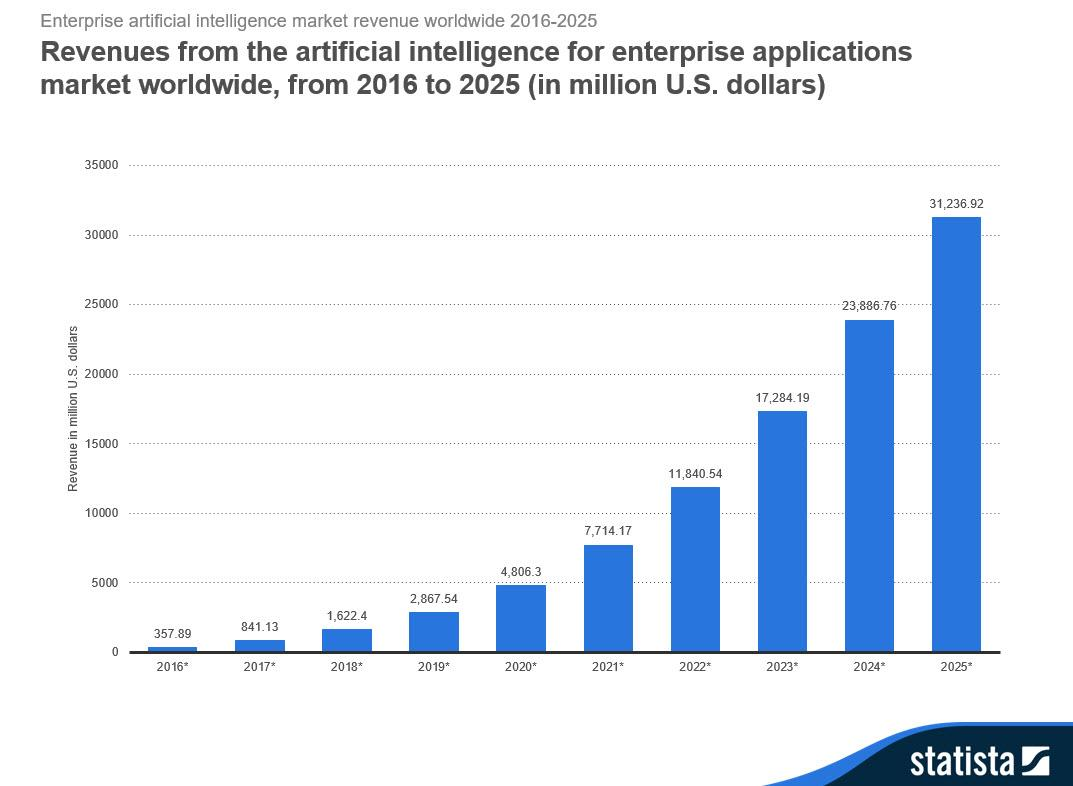
\includegraphics[width=\textwidth]{figures/ai-projections.jpg}
       \caption{Enterprise AI market revenue 2016-2025 (image from \cite{ai-proj}).}
       \label{fig:ai-proj}
   \end{subfigure}%
   ~
   \begin{subfigure}[b]{0.5\textwidth}
       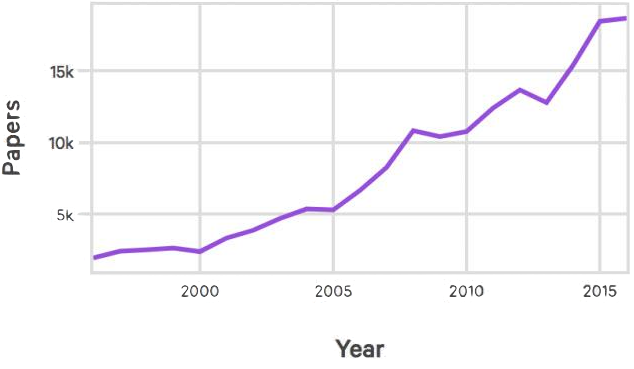
\includegraphics[width=\textwidth]{figures/ai-papers.png}
       \caption{AI papers published per year (image from \cite{ai-papers}).}
       \label{fig:ai-papers}
   \end{subfigure}
\end{figure}

A part of the current EU funding has been allocated to the Human Brain Project (HBP) \cite{hbp}, designated as one of the Horizon 2020 Future and Emerging Technologies Flagship projects with over a billion euros in budget. It is a 10-year initiative launched in 2013 that strives to accelerate the fields of neuroscience, brain-related medicine and computing. The project is broken down into multiple topics, referred to as pillars, one of which is focused on neuromorphic computing to build a novel platform to run neural network simulations. There has never been a unique way of building intelligent systems, and neuromorphic computing is the approach that tries to mimic the morphology of the brain to design hardware in the hope that it will yield the most faithful neural simulations. In the context of HBP, this meant building a novel type of computer with a design directly inspired from the brain which led to the Spiking Neural Network Architecture (SpiNNaker) machine\cite{SpiNNaker-Project}. Spiking neural networks are the neuromorphic version of the traditional artificial neural networks. The latter are "simply" mathematical models trying to approximate the state of the brain, while spiking neural networks will try to reproduce the exact interactions between each brain cell in the hope of getting an even closer approximation. \\

The deliverables of SpiNNaker include a new physical machine, formed of a cluster of neuromorphic printed circuit boards accessible via an online interface for researchers to remotely use. The development process of the machine was iterative, with a single circuit board produced at first which then got assembled in a cluster. For this project, we were fortunate enough to use the first release of the machine: the \textit{102} machine formed of a single circuit board - see Fig.~\ref{fig:spinn3}. The name \textit{102} comes from the machine having approximately $10^2$ cores (72 in fact). The last version of the machine called \textit{106}, meaning it has $10^6 = 1$M cores and there is currently a single version of it (half-finished but functional) at the University of Manchester, where it was built. \\

\begin{figure}[!ht]
   \centering
       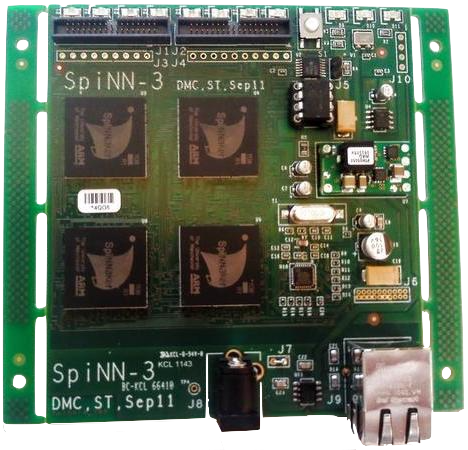
\includegraphics[width=0.7\textwidth]{figures/spin3.png}
       \caption{The SpiNNaker \textit{102} machine, used for prototyping this project (image from \cite{spinn-3}).}
       \label{fig:spinn3}
\end{figure}

These machines present the following hardware characteristics that motivated this project, some of which differ from a classic supercomputer architecture:

\begin{itemize}
\item \textbf{Manycore architecture}: as explained above, the density of cores on the board isthe main design feature inspired from the brain, which has around 86 billions of neural cells \cite{5th-summit}.

\item \textbf{Communication model}: cores communicate through message passing, with messages being small datagrams sent over UDP/IP (72 bits maximum) \cite{ws6}. UDP/IP is a best-effort communication protocol and thus, the sender does not get any guaranty its messages were delivered. This design decision is at the heart of the network layer and is directly inspired from the brain, where a neuron does not get any reception acknowledgement when communicating with neighbouring neurons.

\item \textbf{Communication throughput}: the expected benefit, gained from reducing the message size, was that a greater number of messages could be processed in a second. For cores on the same circuit board, their link can transfer up to 250M bit/s, meaning it could process up to 3M packet/s \cite{ws6}.
\end{itemize}

The details of these hardware specificities will be covered in greater details in the background (section \ref{sec:bg}) of this report. \\

The deliverables of SpiNNaker also include a constellation of specialised software modules that each fulfill a specific mission. Indeed, SpiNNaker is not a regular computer on which users could simply install a Linux distribution and log in. A host machine, connected by Ethernet to SpiNNAker, is needed and pre-compiled binaries can be loaded on selected cores of SpiNNaker from it. This segregation between host and SpiNNaker machine increases the number of software modules needed, which we will cover in greater details in section \ref{sec:sw}. \\

All in all, a SpiNNaker machine can be viewed as a small supercomputer where cores can exchange a considerable amount of small packets at the cost of message delivery reliability. These biology-inspired properties are well suited for spiking neural networks simulations, and illustrate what a neuromorphic computer has the potential to be. It is also these properties that created an opportunity for this project, which we discuss in the next paragraph. \\


\subsection{Objectives}

In order to explore the new opportunities offered by SpiNNaker, we first define the mission statement of this project as follows:

\begin{quote}
\textit{Investigate how we could leverage SpiNNaker for graph processing, using Page Rank as a benchmark, in the hope that it will give a better scalability potential than traditional computers.
}\end{quote}

This project aims to make a contribution to the existing SpiNNaker research by exposing a new application for the machine, since Page Rank has never been ported to the machine before, or at least it never resulted in a publication. Still, alternative applications have already been explored, such as heat equation solving \cite{heat} or Markov Chain Monte Carlo Simulations \cite{markov-on-spinn}, and drawing comparisons with these examples will be interesting in the next sections (\ref{sec:aa}). \\

The reason why graph processing and Page Rank were chosen comes from the data flow of these algorithms.  Indeed, SpiNNaker is optimised for many small-payload exchanges and a single iteration of Page Rank needs to send as many updates as there are edges in its graph. At each iteration, each node sends its weighted rank along its outgoing edges and builds up a new rank by summing the ranks coming from its inbound edges. In SpiNNaker, each of these ranks could be sent as the 32 bits payload of the 72 bits datagram mentioned above. \\

Let us take the concrete example of the Wikipedia page dumps, which are often used as a dataset to bencharmark Page Rank computations. Using the statistics of this study \cite{nayuki} on a dump from early 2014, a graph of all Wikipedia pages was constituted, made of 10M pages (vertices) and 320M links between them (edges). Assuming ranks are encoded with 32 bits, this means at each Page Rank iteration we would need the nodes to exchange $320$M$ \times  32 $bits $= 10$Gb of data. This amount of data could still fit on a single RAM and the computations might not need to be distributed, but for bigger graphs, such as the internet graph indexed by Google, distributing the computation becomes unavoidable. Google claims it has indexed hundreds of billions of pages \cite{google-si} with even more links interconnecting them. This type of graph would require the computation to run in parallel on multiple machines, and the computation being not CPU intensive, the bottleneck probably lies with the communication cost associated with exchanging ranks at each iteration step. To cope with this problem, the biggest edge of SpiNNaker is its low latency interconnect, which would outperform the end-to-end latency of a classic link between two commodity hardware in a data centre. \\

%such as the graph of all Facebook active users, distributing the computations becomes unavoidable. In a dataset from 2011, Facebook had approximatively 721 million users (nodes) for 69 billion friendship links (edges) \cite{fb}. Using the same logic as before, this means the data exchanged per iteration would weigh $69$B$ \times  32 $bits $= 2.2$Tb, and this amount today with Facebook's 2.2 billion active would be even greater \cite{fb-ac-users}.

Consequently, a property we can use to identify algorithms that could scale better on SpiNNaker is the data flow during the computation. If a computation can easily be broken down into \textit{independent} chunks, than this is probably a job more tailored for Map-Reduce \cite{mr}. However, if this is not the case and a lot of state is maintained throughout the computation, with that state needing to be \textit{shared} amongst a lot of workers, than SpiNNaker might be a good alternative. This property is exactly what Page Rank exhibits, and what made it a good choice for a benchmark to confirm this hypothesis about expected improved scalability. \\


\subsection{Contributions}

The contributions from this project are twofold:

\begin{itemize}
\item \textbf{Page Rank simulation framework}: we built the right set of tools to let users run Page Rank simulations effortlessly. Indeed, the software stack of SpiNNaker is quite complex and before implementing anything, a lot of time had to be invested into understanding the SpiNNaker paradigm. These challenges include dependency management of the software modules used, graph vertices mapping to cores, resource allocation, inter-core data routing, algorithm synchronisation barriers between each iteration, resilience to lost packets, results validation and visualisation. All of this complexity is hidden by the framework, and only a list of edges is necessary to quick start a simulation. Details in section \ref{sec:impl}.

\item \textbf{Page Rank scaling}: we demonstrate that Page Rank under SpiNNaker offers better scalability opportunities compared to a traditional PC. We benchmark two implementations of Page Rank: the first one is an (adapted) Python implementation of the well-established \textit{networkx} \cite{networkx} library and second one is a port to SpiNNaker using the framework mentioned above. The performance gain observed shows SpiNNaker allows for a speed-up of a factor of nearly 4 compared to the traditional PC implementation. Details in section \ref{sec:eval}.
\end{itemize}


Here, Page Rank is used as a proof-of-concept but this project aims to show that an entire class of algorithms are well suited for a port to SpiNNaker. The framework provided can easily be extended to support other graph-based algorithm with a data flow similar to Page Rank.
